%(BEGIN_QUESTION)
% Copyright 2014, Tony R. Kuphaldt, released under the Creative Commons Attribution License (v 1.0)
% This means you may do almost anything with this work of mine, so long as you give me proper credit

Undersøk dette skjemaet for et temperaturreguleringssystem for en dampoppvarmet varmeveksler:

$$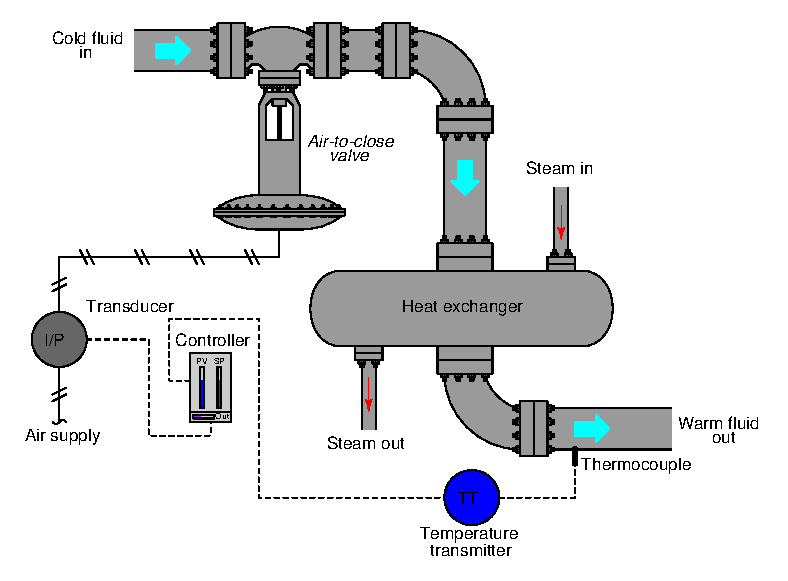
\includegraphics[width=15.5cm]{i00461x01.eps}$$

Bestem hvordan reguleringen av temperaturen inne i beholderen påvirkes hvis termoelementet får brudd (open circuit), slik at temperaturtransmitteren gir høyt signal hele tiden (det vil si TT-utgang $>$ 20 mA). Anta at alle sløyfekomponenter er riktig konfigurert, at regulatoren er godt tunet, og at det har gått betydelig tid siden feilen oppstod. Sammenlign disse forholdene med tilstanden før feilen:

\begin{itemize}
\item{} Reguleringsventilen vil: {\it åpne mer}, {\it lukke mer}, eller {\it forbli i samme posisjon}
\vskip 10pt
\item{} Prosesstemperaturen vil: {\it øke}, {\it synke}, eller {\it være uendret} sammenlignet med før
\end{itemize}

\underbar{file i00461}
%(END_QUESTION)





%(BEGIN_ANSWER)

\begin{itemize}
\item{} Reguleringsventilen vil: {\bf åpne mer}
\vskip 10pt
\item{} Prosesstemperaturen vil: {\bf synke}
\end{itemize}

%(END_ANSWER)





%(BEGIN_NOTES)

{\bf Denne oppgaven er ment for eksamen, ikke arbeidsark!}.

%(END_NOTES)
